\section{Funcionalidades}

O Calopsita é feito utilizando uma arquitetura de plugins. Ou seja, a aplicação tem um núcleo, contendo a parte básica do sistema e todo o resto é feito ou configurado com a criação de plugins, dando um grande poder de customização.
Entre as funcionalidades que fazem parte do núcleo estão a criação e administração de usuários,
projetos, cartões, iterações e ações para log.

O Calopsita, ao contrário de outros sistemas com o mesmo propósito, não possui o conceito de histórias, apenas de cartões. Isso foi feito pensando em trazer maior grau de customização para os usuários, uma vez que cartões podem ter subcartões. Essa funcionalidade permite uma hierarquia tão profunda quanto se deseje, e permite que o projeto seja visto no nível de detalhe mais apropriado pra cada envolvido no projeto, seja um gerente, desenvolvedor, product owner, etc.

A arquitetura de plugins

\begin{figure}[htbp]
  \centering
  \fbox{
    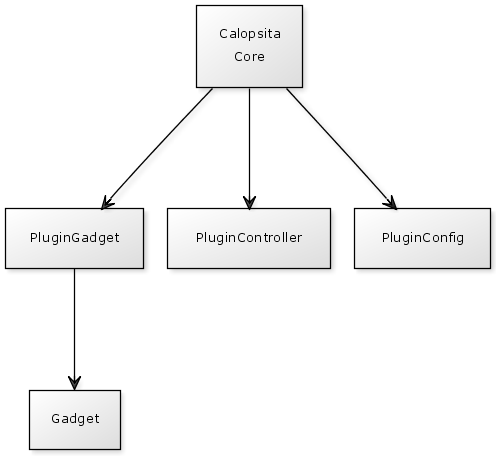
\includegraphics[width=110mm]{images/plugins_uml.png}
  }
  \caption{Arquitetura de plugins}
\end{figure}

PluginConfig -> menu
PluginController -> logica + views
Gadget -> info nos cartoes

tudo isso ligado ao core por injeção de dependencia do spring


Esses são os plugins que implementamos:
priorizacao
burnup
burn down
marcar horas
estimativa
templates de metodologias
templates de cartão


